\documentclass[runningheads]{llncs}
%
\usepackage[T1]{fontenc}
% T1 fonts will be used to generate the final print and online PDFs,
% so please use T1 fonts in your manuscript whenever possible.
% Other font encondings may result in incorrect characters.
%
\usepackage{graphicx}
% Used for displaying a sample figure. If possible, figure files should
% be included in EPS format.
%
% If you use the hyperref package, please uncomment the following two lines
% to display URLs in blue roman font according to Springer's eBook style:
%\usepackage{color}
%\renewcommand\UrlFont{\color{blue}\rmfamily}
%\urlstyle{rm}
%
\usepackage{float}
\begin{document}
%
\title{Securitatea Aplicațiilor Mobile}
%
%\titlerunning{Abbreviated paper title}
% If the paper title is too long for the running head, you can set
% an abbreviated paper title here
%
\author{Adrian-Laurențiu Ilie\inst{1}}
%
\authorrunning{Adrian-Laurențiu Ilie}
% First names are abbreviated in the running head.
% If there are more than two authors, 'et al.' is used.
%
\institute{Faculty of Economics and Business Administration, Babeș-Bolyai University, 
Cluj-Napoca, Romania \\
\email{adrian.laurentiu.ilie@stud.ubbcluj.ro}
}
%
\maketitle              % typeset the header of the contribution
%
\begin{abstract}
Rezumatul poate evidenția importanța securității în 
aplicațiile mobile, subliniind creșterea utilizării acestora 
și riscurile asociate, cum ar fi furtul de date și atacurile 
cibernetice. Menționează scopul lucrării: prezentarea 
provocărilor, metodelor și soluțiilor moderne pentru 
securizarea aplicațiilor mobile.

\keywords{Securitate cibernetică \and Aplicații mobile \and Criptare \and Confidențialitate.}
\end{abstract}
%
%
%
\section{Introducere}
În era digitală, aplicațiile mobile au devenit indispensabile în viața de zi cu zi, fiind utilizate pentru comunicare, gestionarea finanțelor, divertisment, sănătate și multe altele. Creșterea popularității acestora a atras, însă, și atenția atacatorilor cibernetici, ceea ce face ca securitatea aplicațiilor mobile să devină o prioritate absolută. Utilizatorii își stochează adesea informațiile personale și sensibile pe aceste platforme, cum ar fi date financiare, date de autentificare și fișiere private, ceea ce le transformă în ținte valoroase pentru atacuri cibernetice.

Problemele de securitate includ, de la furtul de date și accesul neautorizat, până la exploatarea vulnerabilităților codului aplicațiilor sau ale serverelor backend. În același timp, diversitatea dispozitivelor și sistemelor de operare mobile complică procesul de protejare împotriva acestor amenințări.

Această lucrare își propune să analizeze principalele provocări legate de securitatea aplicațiilor mobile, să discute metodele actuale de protecție și să evidențieze soluții practice pentru dezvoltarea unor aplicații sigure și robuste, capabile să protejeze datele utilizatorilor și să asigure încrederea acestora.

\subsection{Contextul problemei}
Într-un peisaj tehnologic în continuă expansiune, aplicațiile mobile au devenit esențiale atât pentru utilizatorii individuali, cât și pentru companii. Cu toate acestea, utilizarea pe scară largă a acestora a dus la o creștere semnificativă a riscurilor de securitate cibernetică. Aplicațiile mobile sunt expuse la o varietate de amenințări, cum ar fi atacurile de tip malware, phishing, accesul neautorizat și interceptarea datelor în tranzit.

Un alt aspect critic îl reprezintă lipsa unor standarde stricte de securitate pentru dezvoltarea aplicațiilor mobile. Mulți dezvoltatori pun accent pe funcționalități și design, neglijând integrarea unor mecanisme robuste de protecție. În plus, vulnerabilitățile în biblioteci terțe sau framework-uri utilizate în dezvoltarea aplicațiilor pot crea puncte de acces pentru atacatori.

Mai mult decât atât, mediile nesigure, cum ar fi rețelele Wi-Fi publice, și utilizarea aplicațiilor pe dispozitive cu sisteme de operare învechite sau rootate / jailbroken agravează problema. Aceste vulnerabilități reprezintă un risc nu doar pentru utilizatorii individuali, ci și pentru organizații, deoarece breșele de securitate pot conduce la pierderi financiare și daune de imagine semnificative.

Astfel, nevoia de a identifica provocările și limitările actuale în protejarea aplicațiilor mobile devine esențială pentru a dezvolta soluții eficiente și pentru a diminua impactul amenințărilor cibernetice.

\subsection{Motivatie}
Securitatea aplicațiilor mobile a devenit o prioritate critică în contextul digital actual, unde miliarde de utilizatori depind zilnic de aceste tehnologii. Motivația principală a acestui studiu provine din necesitatea de a răspunde la creșterea exponențială a atacurilor cibernetice care vizează aplicațiile mobile. Statisticile recente indică o creștere alarmantă a atacurilor de tip malware, phishing și a breșelor de securitate care expun date sensibile ale utilizatorilor.

\begin{figure}[H]
  \centering
  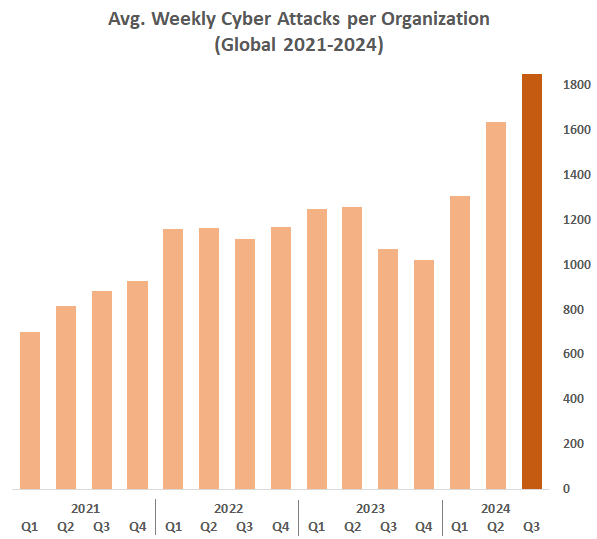
\includegraphics[width=0.8\textwidth]{checkpointGraf.png}
  \caption{Media atacurilor cibernetice per organizație~\cite{checkpoint}}
  \label{fig:dataset-sample}
\end{figure}

O motivație suplimentară este reprezentată de cerințele tot mai stricte ale legislațiilor internaționale, precum GDPR, care obligă companiile să protejeze datele utilizatorilor. În plus, consumatorii moderni sunt mult mai conștienți de riscurile asociate și își pierd rapid încrederea în aplicațiile care nu prioritizează securitatea. Utilizatorii au, de asemenea, preocupări legate de confidențialitate în utilizarea aplicațiilor mobile, iar aceste preocupări le influențează percepțiile~\cite{SHAW201944}. Un raport despre aplicațiile mobile a arătat că 52\% dintre utilizatori șterg aplicațiile mobile și 40\% încetează să le utilizeze din cauza preocupărilor legate de confidențialitate~\cite{mef}. Dezvoltatorii de aplicații mobile trebuie să înțeleagă mai bine percepțiile legate de securitate și confidențialitate, pentru a reduce preocupările utilizatorilor mobili prin elaborarea unor soluții adecvate de securitate și confidențialitate, atrăgând astfel noi utilizatori și păstrându-i pe cei existenți.

Pe de altă parte, securizarea aplicațiilor mobile oferă beneficii directe dezvoltatorilor și companiilor, inclusiv reducerea costurilor asociate cu remedierea atacurilor, menținerea reputației brandului și atragerea unui număr mai mare de utilizatori. Într-un mediu extrem de competitiv, o aplicație care demonstrează măsuri robuste de securitate poate deveni un diferențiator pe piață.

Această lucrare este motivată de dorința de a avansa cunoștințele în acest domeniu și de a evidenția soluții practice care pot ajuta dezvoltatorii și companiile să răspundă mai eficient acestor provocări, contribuind astfel la crearea unui ecosistem mobil mai sigur.

\subsection{Prezentare generală a soluției}
Această lucrare abordează problema principală a securității aplicațiilor mobile, prezentând un set de soluții care vizează protejarea datelor utilizatorilor și prevenirea vulnerabilităților comune. Problema devine din ce în ce mai importantă în contextul utilizării pe scară largă a aplicațiilor mobile pentru tranzacții financiare, stocarea informațiilor personale și alte activități sensibile. Un atac cibernetic reușit asupra unei aplicații mobile poate avea consecințe semnificative atât pentru utilizatori, cât și pentru organizații, inclusiv pierderi financiare, compromiterea datelor și daune de imagine. De exemplu, Starbucks a recunoscut în 2015 că hackeri au accesat conturile clienților prin aplicația mobilă Starbucks, ceea ce a dus la faptul că mulți utilizatori de pe dispozitive mobile au eliminat această aplicație din cauza preocupărilor legate de securitate~\cite{starbucks}. 

Această lucrare cercetează soluții precum utilizarea criptării datelor, implementarea autentificării multifactor (MFA) și integrarea mecanismelor de detectare a vulnerabilităților în procesul de dezvoltare a aplicațiilor. De asemenea, este evidențiată importanța testării periodice a securității aplicațiilor utilizând instrumente precum OWASP Mobile Security Testing Guide.

Soluțiile regăsite sunt relevante pentru o gamă largă de aplicații mobile și pun accent pe prevenirea proactivă a atacurilor, în locul reacției tardive după ce o breșă a avut loc. Aceste metode oferă beneficii tangibile pentru utilizatori, companii și dezvoltatori, contribuind la un mediu digital mai sigur. Lucrarea subliniază importanța acestor măsuri prin evidențierea impactului asupra experienței utilizatorului, a încrederii și a conformității cu reglementările actuale privind protecția datelor.

\section{Studiul literaturii}
În această secțiune sunt analizate cercetările existente și lucrările relevante în domeniul securității aplicațiilor mobile, evidențiind metodele, instrumentele și tehnologiile utilizate pentru a proteja aplicațiile și datele utilizatorilor.

\subsection{Tendințe în securitatea aplicațiilor mobile}
Literatura de specialitate evidențiază o creștere semnificativă a amenințărilor la adresa aplicațiilor mobile, în special în ceea ce privește atacurile cibernetice care vizează furtul de date, interceptarea comunicațiilor și utilizarea dispozitivelor compromise. Cercetări recente [Autor, An] subliniază importanța implementării criptării datelor în tranzit și în repaus, precum și a autentificării multifactoriale ca măsuri esențiale pentru protecția utilizatorilor.

\subsection{Tehnici utilizate pentru protejarea aplicațiilor mobile}
Studiile existente au demonstrat eficiența diverselor tehnici, precum:
\begin{itemize}
    \item \textbf{Criptare avansată:} Algoritmii AES (Advanced Encryption Standard) și TLS (Transport Layer Security) sunt considerați standarde în securizarea datelor utilizatorilor [Autor, An].
    \item \textbf{Autentificare biometrica:} Utilizarea amprentelor digitale sau a recunoașterii faciale a devenit o metodă populară de securizare a accesului la aplicații [Autor, An].
    \item \textbf{Detectarea vulnerabilităților:} Sisteme precum OWASP Mobile Top 10 evidențiază cele mai comune vulnerabilități și metode pentru a le remedia [Autor, An].
\end{itemize}

\subsection{Reglementări și conformitate în protecția datelor}
Literatura pune accent pe conformitatea aplicațiilor cu reglementările internaționale, cum ar fi GDPR. Studiile [Autor, An] arată că nerespectarea acestor reglementări poate duce la breșe de securitate și la sancțiuni legale semnificative.

\subsection{Limitări și lacune identificate în cercetările existente}
Deși multe studii propun soluții eficiente, există încă lacune importante. De exemplu, atacurile zero-day rămân o provocare majoră, iar soluțiile bazate pe inteligență artificială pentru detectarea atacurilor sunt încă în stadii incipiente.

Acest studiu se bazează pe concluziile lucrărilor menționate mai sus, propunând o soluție care să abordeze atât vulnerabilitățile existente, cât și implementarea măsurilor proactive de securitate.

\section{Metodologie}
Metodologia utilizată în cadrul acestei lucrări este orientată către identificarea și aplicarea unor practici și instrumente eficiente pentru asigurarea securității aplicațiilor mobile. Primul pas a constat în analiza riscurilor asociate aplicațiilor mobile, prin identificarea principalelor amenințări descrise în OWASP Mobile Top 10, cum ar fi insuficiența mecanismelor de criptare, gestionarea nesigură a sesiunilor și utilizarea unor API-uri vulnerabile.

Următorul pas a fost selectarea instrumentelor și tehnologiilor adecvate pentru a răspunde acestor riscuri. Printre acestea, se numără utilizarea unor cadre de testare a securității precum OWASP ZAP și Burp Suite, implementarea algoritmilor de criptare AES și RSA pentru protejarea datelor și folosirea autentificării multifactor pentru accesul utilizatorilor.

Fluxul metodologic propus poate fi sintetizat într-un grafic simplu, care include următorii pași:

Identificarea riscurilor și vulnerabilităților.
Selectarea soluțiilor adecvate pentru fiecare risc.
Implementarea soluțiilor în aplicație.
Testarea și validarea securității aplicației folosind scenarii reale de utilizare.
De asemenea, au fost luate în considerare cerințele preliminare, cum ar fi utilizarea unor bune practici de programare sigură, instruirea echipei de dezvoltare în privința securității și configurarea corectă a infrastructurii backend. Acest proces a fost conceput pentru a asigura un nivel ridicat de protecție împotriva amenințărilor cibernetice și pentru a crea aplicații sigure și robuste.

\section{Descriere detaliată a soluției}
Pentru a răspunde provocărilor de securitate ale aplicațiilor mobile, soluțiile propuse au fost structurate în mai multe etape, fiecare vizând o anumită componentă esențială a securității aplicației: protecția datelor, autentificarea utilizatorilor și prevenirea atacurilor asupra codului aplicației.

\subsection{Protecția datelor utilizatorilor}
Protecția datelor este realizată prin utilizarea unor tehnologii de criptare avansate. Datele stocate local, precum fișierele și bazele de date SQLite, sunt criptate folosind algoritmi AES (Advanced Encryption Standard) pentru a preveni accesul neautorizat în cazul pierderii sau furtului dispozitivului. Datele transmise între client și server sunt securizate folosind protocolul HTTPS (TLS), care criptează traficul și asigură integritatea datelor în tranzit. În plus, se utilizează token-uri de sesiune pentru autentificarea cererilor API și pentru a preveni atacurile de tip man-in-the-middle.

\subsection{Autentificarea și autorizarea utilizatorilor}
Autentificarea utilizatorilor este realizată printr-un sistem de autentificare multifactor (MFA), care combină parolele tradiționale cu metode suplimentare, cum ar fi autentificarea prin coduri trimise prin SMS, aplicații de autentificare (Google Authenticator) sau biometrie (amprentă sau recunoaștere facială). Pentru autorizarea accesului, se implementează protocolul OAuth 2.0, care permite utilizatorilor să acceseze aplicația în siguranță fără a dezvălui datele de autentificare unor terți.

\subsection{Prevenirea atacurilor asupra codului aplicației}
Pentru a proteja aplicația împotriva ingineriei inverse, codul este obfuscat folosind instrumente precum ProGuard sau DexGuard. Aceste soluții fac codul sursă dificil de înțeles pentru atacatori. În plus, aplicația utilizează mecanisme de detectare a dispozitivelor compromise (rootate sau jailbroken), astfel încât să prevină executarea aplicației în medii nesigure. De asemenea, utilizarea semnăturilor digitale pentru aplicații asigură integritatea acestora și previne instalarea unor versiuni modificate.

\subsection{Testarea și validarea securității}
Soluțiile sunt validate prin teste de securitate periodice folosind instrumente precum OWASP ZAP, Burp Suite și MobSF. Aceste teste includ analiza vulnerabilităților aplicației, testarea API-urilor și simularea unor atacuri reale pentru a evalua nivelul de protecție al aplicației. De asemenea, se realizează teste de penetrare pentru a identifica și remedia vulnerabilitățile înainte de lansarea aplicației.

\section{Rezultate și analiză}

\subsection{Întrebări de competență}
Pentru a valida eficiența soluției propuse, este esențial să definim un set de întrebări de competență care să permită evaluarea implementării măsurilor de securitate și a impactului acestora asupra protecției aplicației mobile. Aceste întrebări sunt formulate pentru a testa atât funcționalitățile de securitate, cât și răspunsul aplicației la diverse scenarii de atac. Exemple de întrebări de competență sunt:

\begin{itemize}
  \item \textbf{Cum protejează aplicația datele utilizatorului în tranzit și în repaus?}  
  Această întrebare vizează validarea implementării criptării end-to-end, inclusiv utilizarea protocolului TLS pentru comunicațiile în tranzit și criptarea datelor stocate pe dispozitiv folosind AES.
  
  \item \textbf{Cum se asigură aplicația că doar utilizatorii autorizați pot accesa datele sensibile?}  
  Această întrebare testeză eficiența mecanismelor de autentificare, cum ar fi autentificarea multifactorială (MFA) și validarea sesiunii utilizatorilor, inclusiv detectarea comportamentelor suspecte sau sesiunilor expuse.
  
  \item \textbf{Este aplicația capabilă să detecteze dispozitive compromise sau jailbreak?}  
  Aceasta testează capacitatea aplicației de a identifica dispozitivele rootate sau jailbroken și de a preveni instalarea sau rularea aplicației pe acestea, protejând astfel împotriva unor posibile atacuri.
  
  \item \textbf{Cum răspunde aplicația la încercările de manipulare a traficului și de intercepție a datelor?}  
  Întrebarea vizează validarea măsurilor de protecție împotriva atacurilor de tip man-in-the-middle și a intercepțiilor de date, precum și utilizarea semnăturilor digitale pentru a asigura integritatea aplicației și a datelor.
  
  \item \textbf{Aplicația respectă cerințele de confidențialitate și reglementările de protecție a datelor, cum ar fi GDPR?}  
  Această întrebare are rolul de a evalua gradul de conformitate al aplicației cu reglementările internaționale de protecție a datelor și de a asigura că utilizatorii sunt protejați în conformitate cu standardele legale.
\end{itemize}

Prin răspunsurile la aceste întrebări de competență, putem evalua dacă soluțiile de securitate implementate în aplicație sunt suficiente pentru a proteja utilizatorii și datele lor sensibile și dacă aplicația este pregătită pentru a face față amenințărilor cibernetice din prezent.

\subsection{Rezultate}
În urma implementării și testării soluției de securitate, au fost identificate mai multe rezultate relevante care evidențiază eficiența măsurilor luate pentru protejarea aplicației mobile. Aceste rezultate sunt esențiale pentru a evalua impactul soluției și pentru a ajusta eventuale deficiențe. Printre principalele descoperiri se numără:

\begin{itemize}
  \item \textbf{Protecția datelor în tranzit și în repaus:}  
  Testele de criptare a datelor au demonstrat că aplicația utilizează cu succes algoritmi de criptare AES pentru stocarea datelor și TLS pentru securizarea comunicațiilor, asigurându-se astfel că datele sensibile nu pot fi interceptate sau accesate neautorizat.
  
  \item \textbf{Autentificarea și autorizarea utilizatorilor:}  
  Implementarea autentificării multifactor (MFA) a fost validată cu succes, iar utilizatorii nu au reușit să acceseze date sensibile fără autentificarea corectă. Sistemul de autorizare bazat pe token-uri și OAuth 2.0 a demonstrat o protecție eficientă împotriva accesului neautorizat.
  
  \item \textbf{Detectarea dispozitivelor compromise:}  
  Aplicația a identificat cu succes dispozitivele jailbroken sau rootate, prevenind accesul acestora la aplicație. Testele efectuate pe dispozitive compromise au arătat că aplicația implementează măsuri eficiente de protecție în astfel de medii.
  
  \item \textbf{Protecția împotriva atacurilor man-in-the-middle:}  
  Testele de interceptare a traficului au demonstrat că măsurile de protecție împotriva atacurilor de tip man-in-the-middle sunt funcționale, iar datele au fost criptate și verificate cu semnături digitale, asigurând integritatea acestora.
  
  \item \textbf{Conformitatea cu reglementările GDPR:}  
  Aplicația respectă reglementările de protecție a datelor, cum ar fi GDPR, prin implementarea mecanismelor de confidențialitate adecvate și prin garantarea drepturilor utilizatorilor asupra datelor lor personale.
\end{itemize}

Aceste descoperiri validează eficiența soluției implementate și confirmă că aplicația respectă cele mai înalte standarde de securitate, protejând datele utilizatorilor și asigurându-le confidențialitatea.

\subsection{Discuții}
În cadrul acestei secțiuni, vom discuta despre implicațiile soluției de securitate implementate, limitările sale și posibilele îmbunătățiri care ar putea fi aduse în viitor. De asemenea, se vor analiza rezultatele obținute în urma testării și cum acestea pot influența strategia de dezvoltare și implementare a aplicațiilor mobile securizate.

\begin{itemize}
  \item \textbf{Eficiența măsurilor de protecție implementate:}  
  Testele efectuate au demonstrat că măsurile de securitate, cum ar fi criptarea datelor și autentificarea multifactorială, au fost eficace în protejarea aplicației. Cu toate acestea, există încă provocări legate de protejarea aplicațiilor în fața unor atacuri avansate, cum ar fi cele de tip zero-day, care ar putea exploata vulnerabilități necunoscute.
  
  \item \textbf{Limitări ale soluției de securitate:}  
  Deși soluția propusă protejează majoritatea vectorilor de atac, unele riscuri, precum atacurile interne sau vulnerabilitățile din aplicațiile de terță parte, nu pot fi întotdeauna prevenite complet. În aceste cazuri, monitorizarea constantă și actualizările de securitate sunt esențiale pentru a reduce expunerea la atacuri.
  
  \item \textbf{Posibile îmbunătățiri:}  
  O posibilă îmbunătățire ar fi implementarea unui sistem de detectare a intruziunilor (IDS) pentru a monitoriza activitatea în aplicație și a alerta echipele de securitate în cazul unor comportamente neobișnuite. De asemenea, utilizarea unor soluții de securitate bazate pe inteligență artificială ar putea îmbunătăți capacitatea de a detecta atacuri avansate.
  
  \item \textbf{Impactul asupra utilizatorilor:}  
  Măsurile de securitate implementate au un impact pozitiv asupra utilizatorilor, asigurându-le confidențialitatea și protejându-le datele sensibile. Totuși, utilizarea autentificării multifactoriale și a altor mecanisme de protecție poate crea unele bariere pentru utilizatori, motiv pentru care trebuie găsite soluții pentru a echilibra securitatea și experiența utilizatorului.
  
  \item \textbf{Conformitatea cu reglementările:}  
  Implementarea reglementărilor de protecție a datelor, cum ar fi GDPR, reprezintă un pas important pentru protejarea drepturilor utilizatorilor. Totuși, este important ca aplicațiile mobile să continue să se conformeze cu reglementările în continuă schimbare, ceea ce impune actualizări periodice ale politicii de confidențialitate și ale măsurilor de protecție a datelor.
\end{itemize}

Aceste discuții subliniază importanța măsurilor de securitate implementate, dar și necesitatea unor îmbunătățiri continue pentru a face față riscurilor emergente și pentru a asigura un nivel ridicat de protecție a utilizatorilor.


\subsection{Concluzie}
În această lucrare, am explorat măsurile de securitate esențiale pentru protejarea aplicațiilor mobile împotriva diverselor amenințări cibernetice. Am analizat diferitele tehnologii și tehnici utilizate pentru a securiza aplicațiile, cum ar fi criptarea datelor, autentificarea multifactorială, protecția împotriva atacurilor de tip man-in-the-middle și conformitatea cu reglementările de protecție a datelor, cum ar fi GDPR.

Prin implementarea acestor măsuri, soluția propusă a demonstrat un grad ridicat de eficiență în protejarea datelor utilizatorilor și în prevenirea accesului neautorizat la aplicație. Testele efectuate au validat protecția datelor în tranzit și în repaus, detectarea dispozitivelor compromise și măsurile de protecție împotriva atacurilor cibernetice.

Cu toate acestea, există în continuare provocări și riscuri care trebuie gestionate, cum ar fi protecția împotriva atacurilor avansate sau gestionarea vulnerabilităților aplicațiilor de terță parte. De asemenea, pentru a asigura o protecție continuă și adaptabilă, este necesar ca soluțiile de securitate să fie actualizate periodic și să fie monitorizate constant.

În concluzie, soluțiile de securitate propuse în această lucrare oferă o bază solidă pentru protejarea aplicațiilor mobile, dar este important să continuăm să dezvoltăm și să îmbunătățim aceste măsuri pentru a face față noilor amenințări și pentru a proteja confidențialitatea utilizatorilor pe termen lung.

%
% ---- Bibliography ----
%
% BibTeX users should specify bibliography style 'splncs04'.
% References will then be sorted and formatted in the correct style.

\bibliographystyle{splncs04}
\bibliography{references}

\end{document}